\documentclass[	%----------------------Preamble---------------------------------------------------%
		11pt,a4paper,	% fontsize and papersize
		twoside,		% double sided layout
		english,		% document language (also numberingsystem)
		f1				% HsH facultie
	]{HsH-report}		% documentclass

\usepackage{color}		% for coloring stuff
\usepackage{siunitx}	% units
\usepackage{listings}
\usepackage{csvsimple}
\usepackage{biblatex}	% bibiography
\addbibresource{src/localBibliography.bib}


\usepackage{lipsum}		% dummy text
\begin{document}

\pagenumbering{Roman}	% duífferent numbering until first chapter
\maketitle				% using personal.tex
\declarationAuthorship

\begin{abstract}
	\lipsum[5-8]
\end{abstract}

\tableofcontents

\cleardoublepage % importand when using double sided layout
\pagenumbering{arabic} % numbering in normal numbers

\chapter{Examples}
	\label{chap: one}
	{\color{red}red text} and {\color{blue}blue text} \\
	different subscripts: \normalsubscripts$R_t$ \upsubscripts$R_t$ \\
	using Units: $R=200\,\milli\ohm + \SI{0.34567453}{\volt\per\metre} - 5\,\si{\second\per\metre\squared}$ \\
	some information\cite{laboranleitung:physik}\\
	german number: $3,5$ english number: $3.5$\\
	\begin{figure}
		
\includegraphics[width=.6\textwidth]{img/lorem-ipsum.jpg}
		\caption{just a random image}
	\end{figure}

	\begin{figure}
		\includegraphics[width=0.6\textwidth, page=2]{plt/build/examplePlot.pdf}
		\caption[centering]{a nice plot}
	\end{figure}

	\begin{figure}
		\graphicspath{{svg/build/}} % double curly brackets needet for unknown reason
		\subfigure[a circuit diagramm]{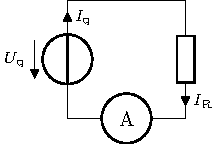
\includegraphics{crc/build/exampleCircuit.pdf}}
		\hspace{2cm}
		\subfigure[made via Inkscape]{\input{svg/build/exampleSVG.pdf_tex}}
		\caption{using two figures}
	\end{figure}

\section{Using formulas}
	\label{sec: formula}
	a numberd formula:
	\begin{equation}
		\label{eq: einhalb} % always lable your stuff
		0,5=\frac{1}{3}
	\end{equation}
	\autoref{eq: einhalb} is nice, but how about multiple lines:
	\begin{equation}
	\begin{split} % you need do nest this
		x &= x^2+3 \\
		\Leftrightarrow 0 &= x^2-x+3 \\
	\end{split}
	\end{equation}
	and how could you align formulas?
	\begin{align}
		x_1 &= 6 &&|\;\mbox{mit } x \in \mathbb{N} \\
		x_2 &= 33+\abs{\frac{1}{4}} &&|\;x_1+3 \\
			&= 33,25 &&\mbox{| don't number everything} \notag \\
		x_3 &= 10^{22}
	\end{align}

\section{formating code}
	\label{sec: code}
	use the listings package:
	% how to skip fist tab??
	\begin{lstlisting}[language=c]
	#include <stdlib.h>
	#include <sdtio.h>

	int main(void) {
		printf("Hello World");
		return 0;
	}
	\end{lstlisting}
	% or input from external file:
	%\lstinputlisting[language=c]{main.c}

\section{CSV files}
	\label{sec: messwerte}
	import a csv as table:\\
	\csvautotabular{csv/bsp.csv}\\
	or do it manualy to get more controll:
	\begin{table}
		\caption{a nice list of numbers}
		\begin{tabular}{c|c}
			first row & second row \\\hline\hline
			\csvreader[
				late after line=\\\hline,
				late after last line=\\\hline
			]{csv/bsp.csv}{}{number: $\csvcoli\,\metre$ & is not \csvcoliii}
		\end{tabular}
	\end{table}

\chapter{attachment}
% manually include a PDF as not numbered section
\textbf{\Large{Messprotokoll oder so}} % just so it'S not empty
\phantomsection % Anker für den Hyperlink
\addcontentsline{toc}{section}{Messprotokoll} % add to table of content
\chaptermark{Messprotokoll}	% change headmark
%\includepdf[pages=-,pagecommand={},width=\paperwidth]{temp.pdf} % comment in to include pdf

\printbibliography
\noindent\begin{minipage}{\textwidth} % prevent automatic pagebreaks
	\listoffigures
	\listoftables
\end{minipage}
\end{document}
